% Reviewed by Gemini 3.1 Pro and Codex gpt-6-astra on 8 October 2026.
% Build: pdflatex, bibtex, pdflatex, pdflatex (references.bib sits beside this file).
\documentclass[10pt,a4paper]{article}
\usepackage[utf8]{inputenc}
\usepackage[margin=0.65in]{geometry}
\usepackage{tikz}
\usepackage{float}
\usepackage{adjustbox}
\usepackage[numbers,sort&compress]{natbib}
\usepackage{url}
\usetikzlibrary{shapes.geometric, arrows.meta, positioning, calc}

\title{\Large\textbf{Playbook: DAG Construction, Refinement, and Causal Attribution}}
\author{\small\textbf{Phase-Based Decision Guide for Causal Modeling Pipeline}}
\date{\small October 2026 (revised 8 October)}

% Compact TikZ Style Definitions
\tikzstyle{startstop} = [
  rectangle,
  rounded corners,
  minimum width=2.8cm,
  minimum height=0.75cm,
  text centered,
  draw=black,
  fill=white,
  text=black,
  text width=2.6cm,
  font=\scriptsize\bfseries
]

\tikzstyle{process} = [
  rectangle,
  minimum width=2.6cm,
  minimum height=0.7cm,
  text centered,
  text width=2.5cm,
  draw=black,
  fill=white,
  text=black,
  font=\scriptsize
]

\tikzstyle{review} = [
  process,
  draw=black,
  line width=1.1pt,
  fill=black!8
]

\tikzstyle{decision} = [
  diamond,
  minimum width=2.2cm,
  minimum height=0.8cm,
  text centered,
  text width=2.0cm,
  draw=black,
  fill=white,
  text=black,
  font=\scriptsize,
  inner sep=1pt
]

\tikzstyle{arrow} = [thick, ->, >=stealth]

\begin{document}

\maketitle
\vspace{-0.6cm}

\section*{Scope \& Prerequisites}
\small \textbf{Scope:} Assumes availability of a labeled dataset suitable for validation. Dataset identification and raw ETL are out of scope. Prediction-only analyses may proceed directly to Predictive Modeling.

\noindent\textbf{Core principle:} No single method establishes a DAG or its attributions. Every step pairs a method with a second method that answers the same question differently, or with a known quantity, and every branch ends in causal review.

\begin{figure}[H]
\centering
\begin{adjustbox}{max width=\textwidth, max height=0.66\textheight}
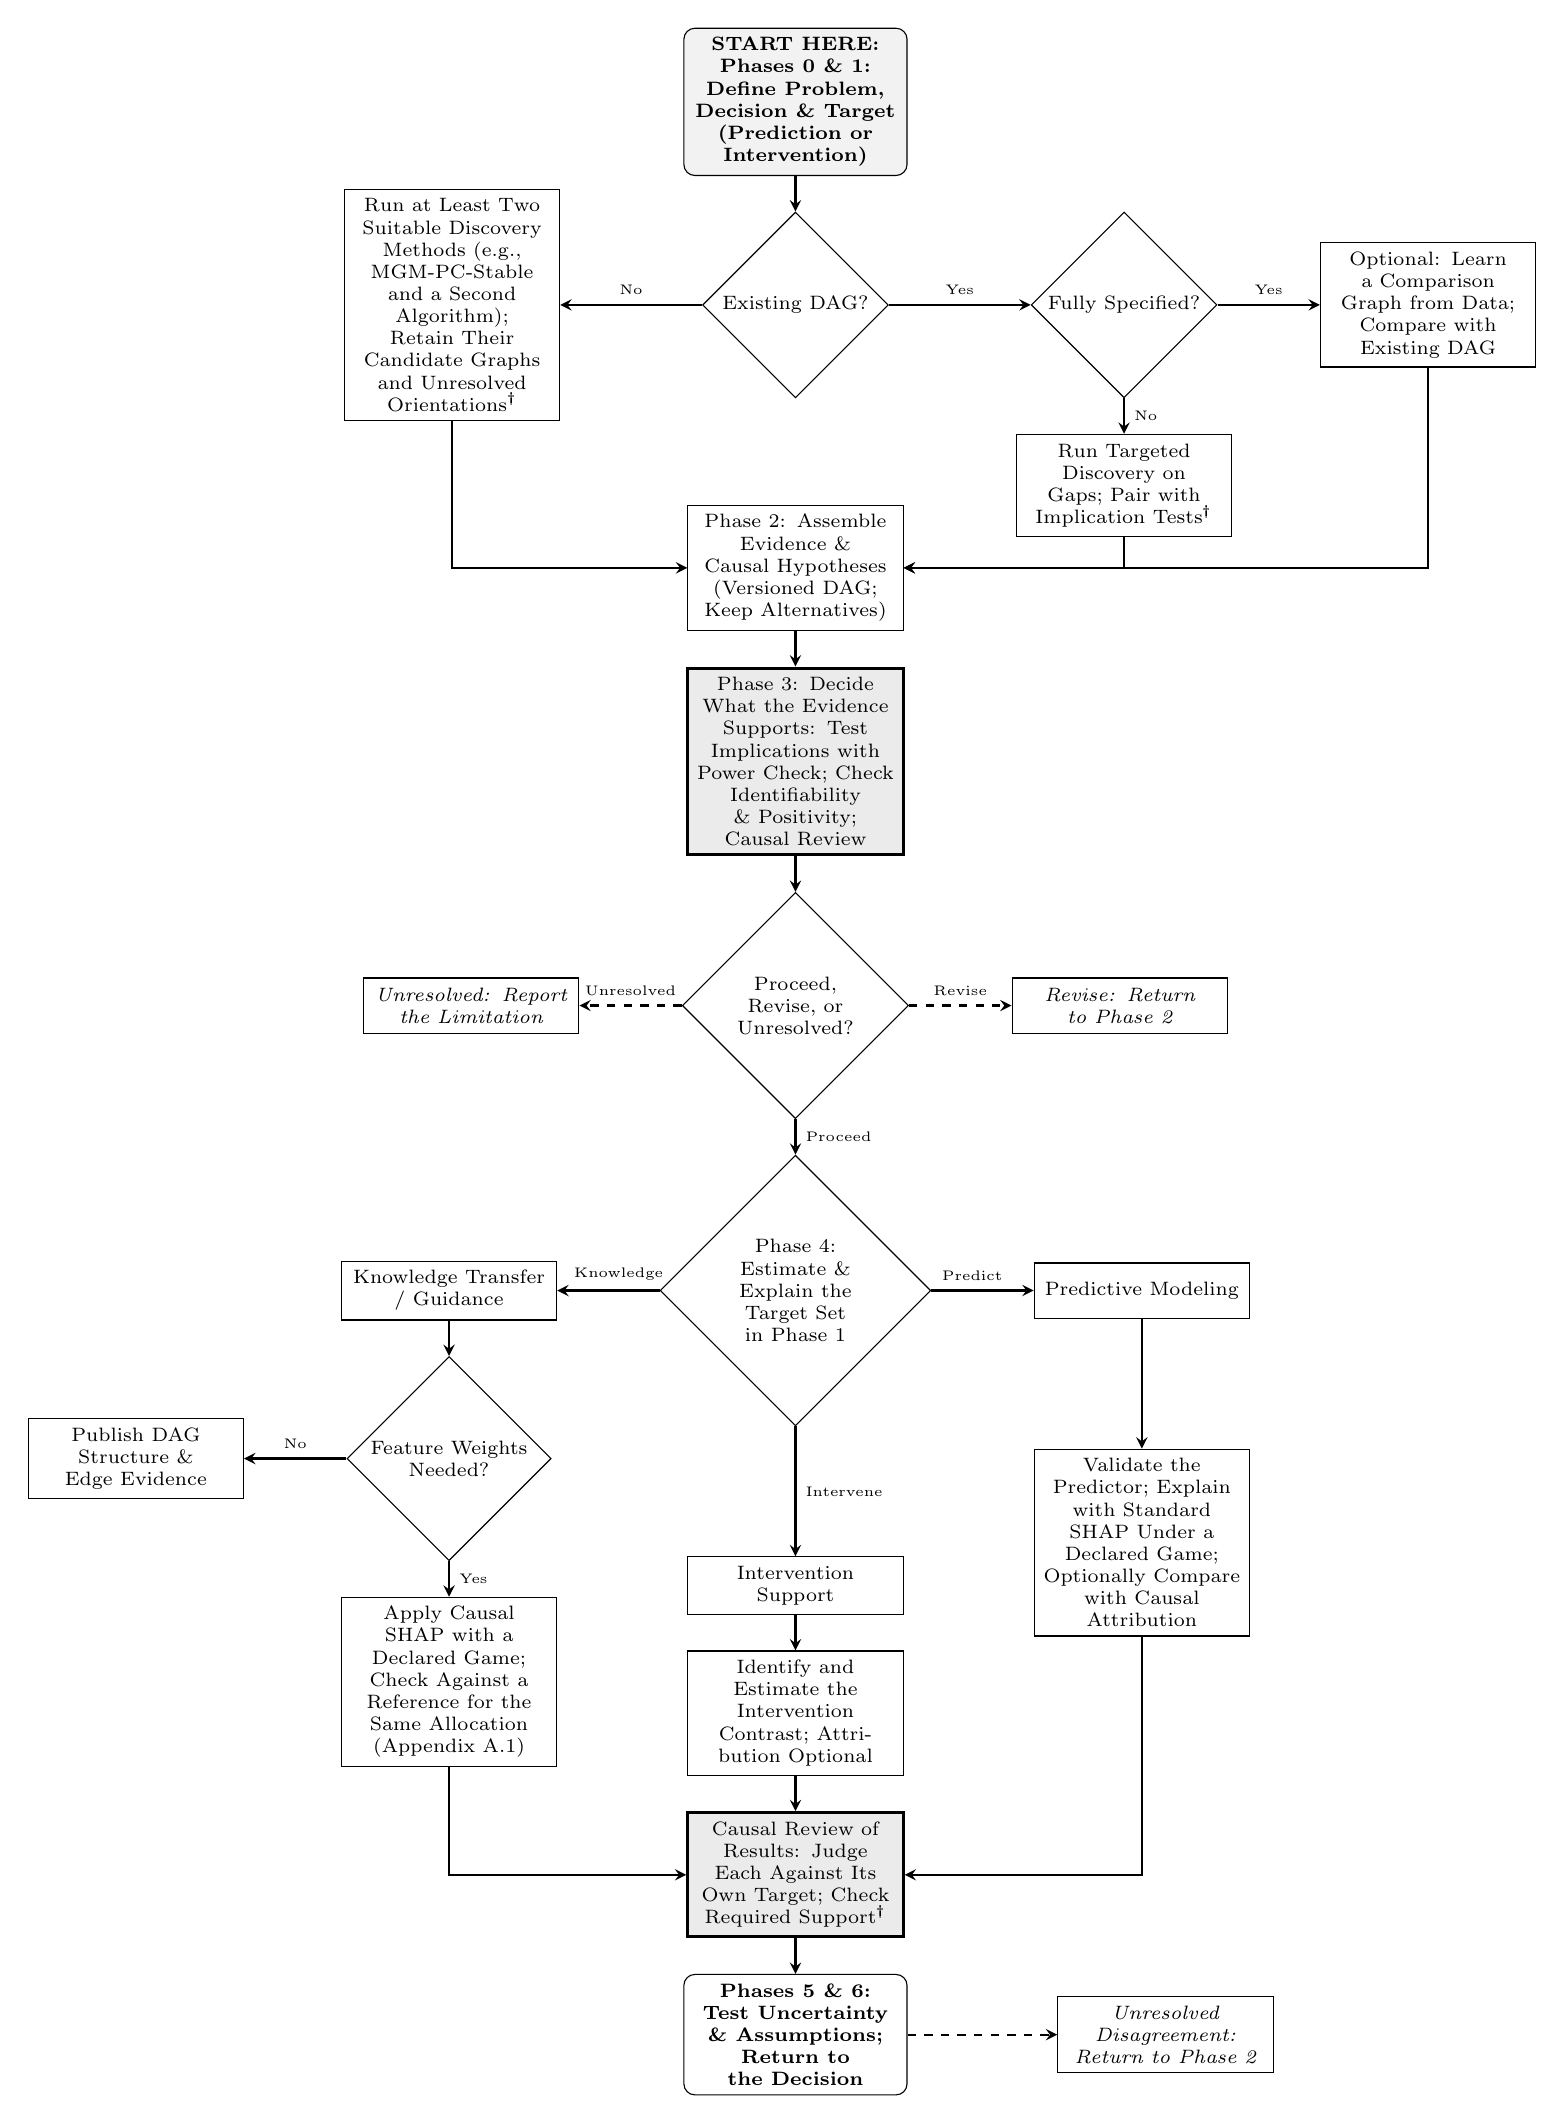
\begin{tikzpicture}[node distance=0.45cm and 1.3cm, auto]

  % --- START NODE / ENTRY POINT ---
  \node (entry) [startstop, fill=black!5] {START HERE:\\Phases 0 \& 1: Define Problem, Decision \& Target (Prediction or Intervention)};

  % --- Module A: Graph State & Refinement (Phases 0-3) ---
  \node (dag_q) [decision, below=of entry] {Existing DAG?};

  \node (discovery) [process, left=of dag_q, xshift=-0.5cm] {Run at Least Two Suitable Discovery Methods (e.g., MGM-PC-Stable and a Second Algorithm); Retain Their Candidate Graphs and Unresolved Orientations\textsuperscript{\dag}};

  \node (spec_q) [decision, right=of dag_q, xshift=0.5cm] {Fully Specified?};

  \node (partial_disc) [process, below=of spec_q] {Run Targeted Discovery on Gaps; Pair with Implication Tests\textsuperscript{\dag}};
  \node (comp_dag) [process, right=of spec_q] {Optional: Learn a Comparison Graph from Data; Compare with Existing DAG};

  \node (synth) [process, below=of dag_q, yshift=-0.9cm] {Phase 2: Assemble Evidence \& Causal Hypotheses (Versioned DAG; Keep Alternatives)};

  \node (phase3) [review, below=of synth] {Phase 3: Decide What the Evidence Supports: Test Implications with Power Check; Check Identifiability \& Positivity; Causal Review};

  \node (conf_dag) [decision, below=of phase3] {Proceed, Revise, or Unresolved?};
  \node (revise_a) [process, right=of conf_dag, font=\scriptsize\itshape] {Revise: Return to Phase 2};
  \node (unres) [process, left=of conf_dag, font=\scriptsize\itshape] {Unresolved: Report the Limitation};

  % Lines for Module A
  \draw [arrow] (entry) -- (dag_q);
  \draw [arrow] (dag_q) -- node[above, font=\tiny] {No} (discovery);
  \draw [arrow] (dag_q) -- node[above, font=\tiny] {Yes} (spec_q);
  \draw [arrow] (spec_q) -- node[right, font=\tiny] {No} (partial_disc);
  \draw [arrow] (spec_q) -- node[above, font=\tiny] {Yes} (comp_dag);

  \draw [arrow] (discovery) |- (synth);
  \draw [arrow] (partial_disc) |- (synth);
  \draw [arrow] (comp_dag) |- (synth);
  \draw [arrow] (synth) -- (phase3);
  \draw [arrow] (phase3) -- (conf_dag);
  \draw [arrow, dashed] (conf_dag) -- node[above, font=\tiny] {Revise} (revise_a);
  \draw [arrow, dashed] (conf_dag) -- node[above, font=\tiny] {Unresolved} (unres);

  % --- Module B: Feature Weight & Downstream Execution (Phase 4) ---
  \node (usecase) [decision, below=of conf_dag] {Phase 4: Estimate \& Explain the Target Set in Phase 1};

  \node (know) [process, left=of usecase] {Knowledge Transfer / Guidance};
  \node (interv) [process, below=of usecase, yshift=-1.2cm] {Intervention Support};
  \node (pred) [process, right=of usecase] {Predictive Modeling};

  \node (attr_q) [decision, below=of know] {Feature Weights Needed?};
  \node (pub_dag) [process, left=of attr_q] {Publish DAG Structure \& Edge Evidence};
  \node (shap_inf) [process, below=of attr_q] {Apply Causal SHAP with a Declared Game; Check Against a Reference for the Same Allocation (Appendix A.1)};

  \node (shap_int) [process, below=of interv] {Identify and Estimate the Intervention Contrast; Attribution Optional};
  \node (shap_pred) [process, below=of pred, yshift=-1.2cm] {Validate the Predictor; Explain with Standard SHAP Under a Declared Game; Optionally Compare with Causal Attribution};

  \node (attr_rev) [review, below=of shap_int] {Causal Review of Results: Judge Each Against Its Own Target; Check Required Support\textsuperscript{\dag}};

  \node (phase5) [startstop, below=of attr_rev] {Phases 5 \& 6:\\Test Uncertainty \& Assumptions; Return to the Decision};

  % Lines for Module B
  \draw [arrow] (conf_dag) -- node[right, font=\tiny] {Proceed} (usecase);
  \draw [arrow] (usecase) -- node[above, font=\tiny, pos=0.4] {Knowledge} (know);
  \draw [arrow] (usecase) -- node[right, font=\tiny] {Intervene} (interv);
  \draw [arrow] (usecase) -- node[above, font=\tiny, pos=0.4] {Predict} (pred);

  \draw [arrow] (know) -- (attr_q);
  \draw [arrow] (attr_q) -- node[above, font=\tiny] {No} (pub_dag);
  \draw [arrow] (attr_q) -- node[right, font=\tiny] {Yes} (shap_inf);

  \draw [arrow] (interv) -- (shap_int);
  \draw [arrow] (pred) -- (shap_pred);

  \draw [arrow] (shap_inf) |- (attr_rev);
  \draw [arrow] (shap_int) -- (attr_rev);
  \draw [arrow] (shap_pred) |- (attr_rev);
  \draw [arrow] (attr_rev) -- (phase5);

  % Iteration: unresolved disagreement returns to the DAG
  \node (revise) [process, right=of phase5, xshift=0.6cm, font=\scriptsize\itshape] {Unresolved Disagreement: Return to Phase 2};
  \draw [arrow, dashed] (phase5) -- (revise);

\end{tikzpicture}
\end{adjustbox}

\vspace{0.1cm}
{\scriptsize Shaded boxes with heavy borders are causal review steps. \textsuperscript{\dag}Recommendation based on reasoning; not tested in the accompanying simulation study. Phase numbers are local to this schematic and differ from manuscript Steps 0--6.}
\end{figure}

\vspace{-0.4cm}

\section*{Key Execution Rules \& Safeguards}
\begin{enumerate}\small
    \item \textbf{Never Rely on One Method:} Pair each method with a second method that answers the same question differently, or check it against a known quantity, such as a simulated ground truth or an effect established in prior studies. Agreement can raise confidence when the methods have different sources of error; agreement alone does not validate the DAG, because methods run on the same data share its selection and measurement error and can succeed for a shared artifact of the data \citep{Lawlor2016,Reisach2021}. PC estimates a Markov equivalence class under its assumptions, so retain unresolved orientations and alternative candidate graphs, and treat intersecting outputs as a stated precision-over-recall choice rather than a default \citep{Maathuis2009}; use tests suited to the variable types \citep{Sedgewick2019}. Disagreement goes to causal review rather than being settled by either method alone.
    \item \textbf{Represent Selection Explicitly:} In a selected cohort, some implications of a correct DAG fail because of how the cohort was selected, not because the DAG is wrong. Draw a selection indicator with arrows from its causes, and treat the analyzed cohort as conditioned on it, before testing implications \citep{HernanSelection2004}.
    \item \textbf{Check Power Before Trusting a Pass:} Implication tests and discovery may have low power for rare exposures, especially in small samples \citep{Textor2016}. Rejection challenges the graph or the testing assumptions; non-rejection does not confirm the graph or support a present edge. Account for graph selection when reusing discovery data for inference \citep{Chang2026}.
    \item \textbf{Sparse Nodes Limit Attribution Too:} Rare exposures can make attribution estimates unstable. Check support for the chosen game; distinguish non-identification from finite-sample bias or imprecision, and do not infer unimportance from either \citep{Petersen2012}.
    \item \textbf{Ordering Alone Does Not Propagate Interventions:} In our matched full-DAG comparison, restricting feature orders produced no detected improvement in intervention-ranking agreement. The separate prototype using known mechanisms showed higher agreement, provisionally; its order law and computational budget also differed. Restricting players to assumed ancestors excludes non-ancestors by construction \citep{Heskes2020,Jung2022,Frye2020}.
    \item \textbf{Causal Attribution Is Only as Good as Its Inputs:} Causal attribution methods use method-specific causal information, such as order constraints or graph structure, with mechanisms where required \citep{Frye2020,Heskes2020,Jung2022}. Errors in those inputs carry into the attributions. Report sensitivity to the retained alternative graphs.\textsuperscript{\dag}
    \item \textbf{Look for Positivity Gaps in the Target's Support:} If the contrast requires exposure within a stratum where it cannot occur, such as a drug never used in one era, it is not identified from those data without additional assumptions \citep{Petersen2012}. Inspect the support the target requires before trusting its attribution; depth itself is not the criterion.
    \item \textbf{Causal Review Closes Every Branch:} A clinical team reviews structure and attributions together; unresolved disagreement returns the analysis to the DAG.\textsuperscript{\dag}
\end{enumerate}

\bibliographystyle{unsrtnat}
\bibliography{references}

\end{document}
